\documentclass{article}
\usepackage[T1]{fontenc}
\usepackage[utf8]{inputenc}
\usepackage[a4paper,top=3.5cm,left=3cm,right=3cm,bottom=2.5cm]{geometry}
\usepackage[brazil]{babel}
\usepackage{graphicx}
\usepackage{hyperref}
\usepackage{fancyhdr}
\usepackage{background}
\usepackage[a4paper,top=3.5cm,left=3cm,right=3cm,bottom=2.5cm]{geometry}
\usepackage{lmodern}

%Configurando a path das imagens
\graphicspath{{../../imagens/capitulo3/}}


%Configurando a imagem de background
\backgroundsetup{
scale=1,
angle=0,
opacity=0.4,
contents={%
  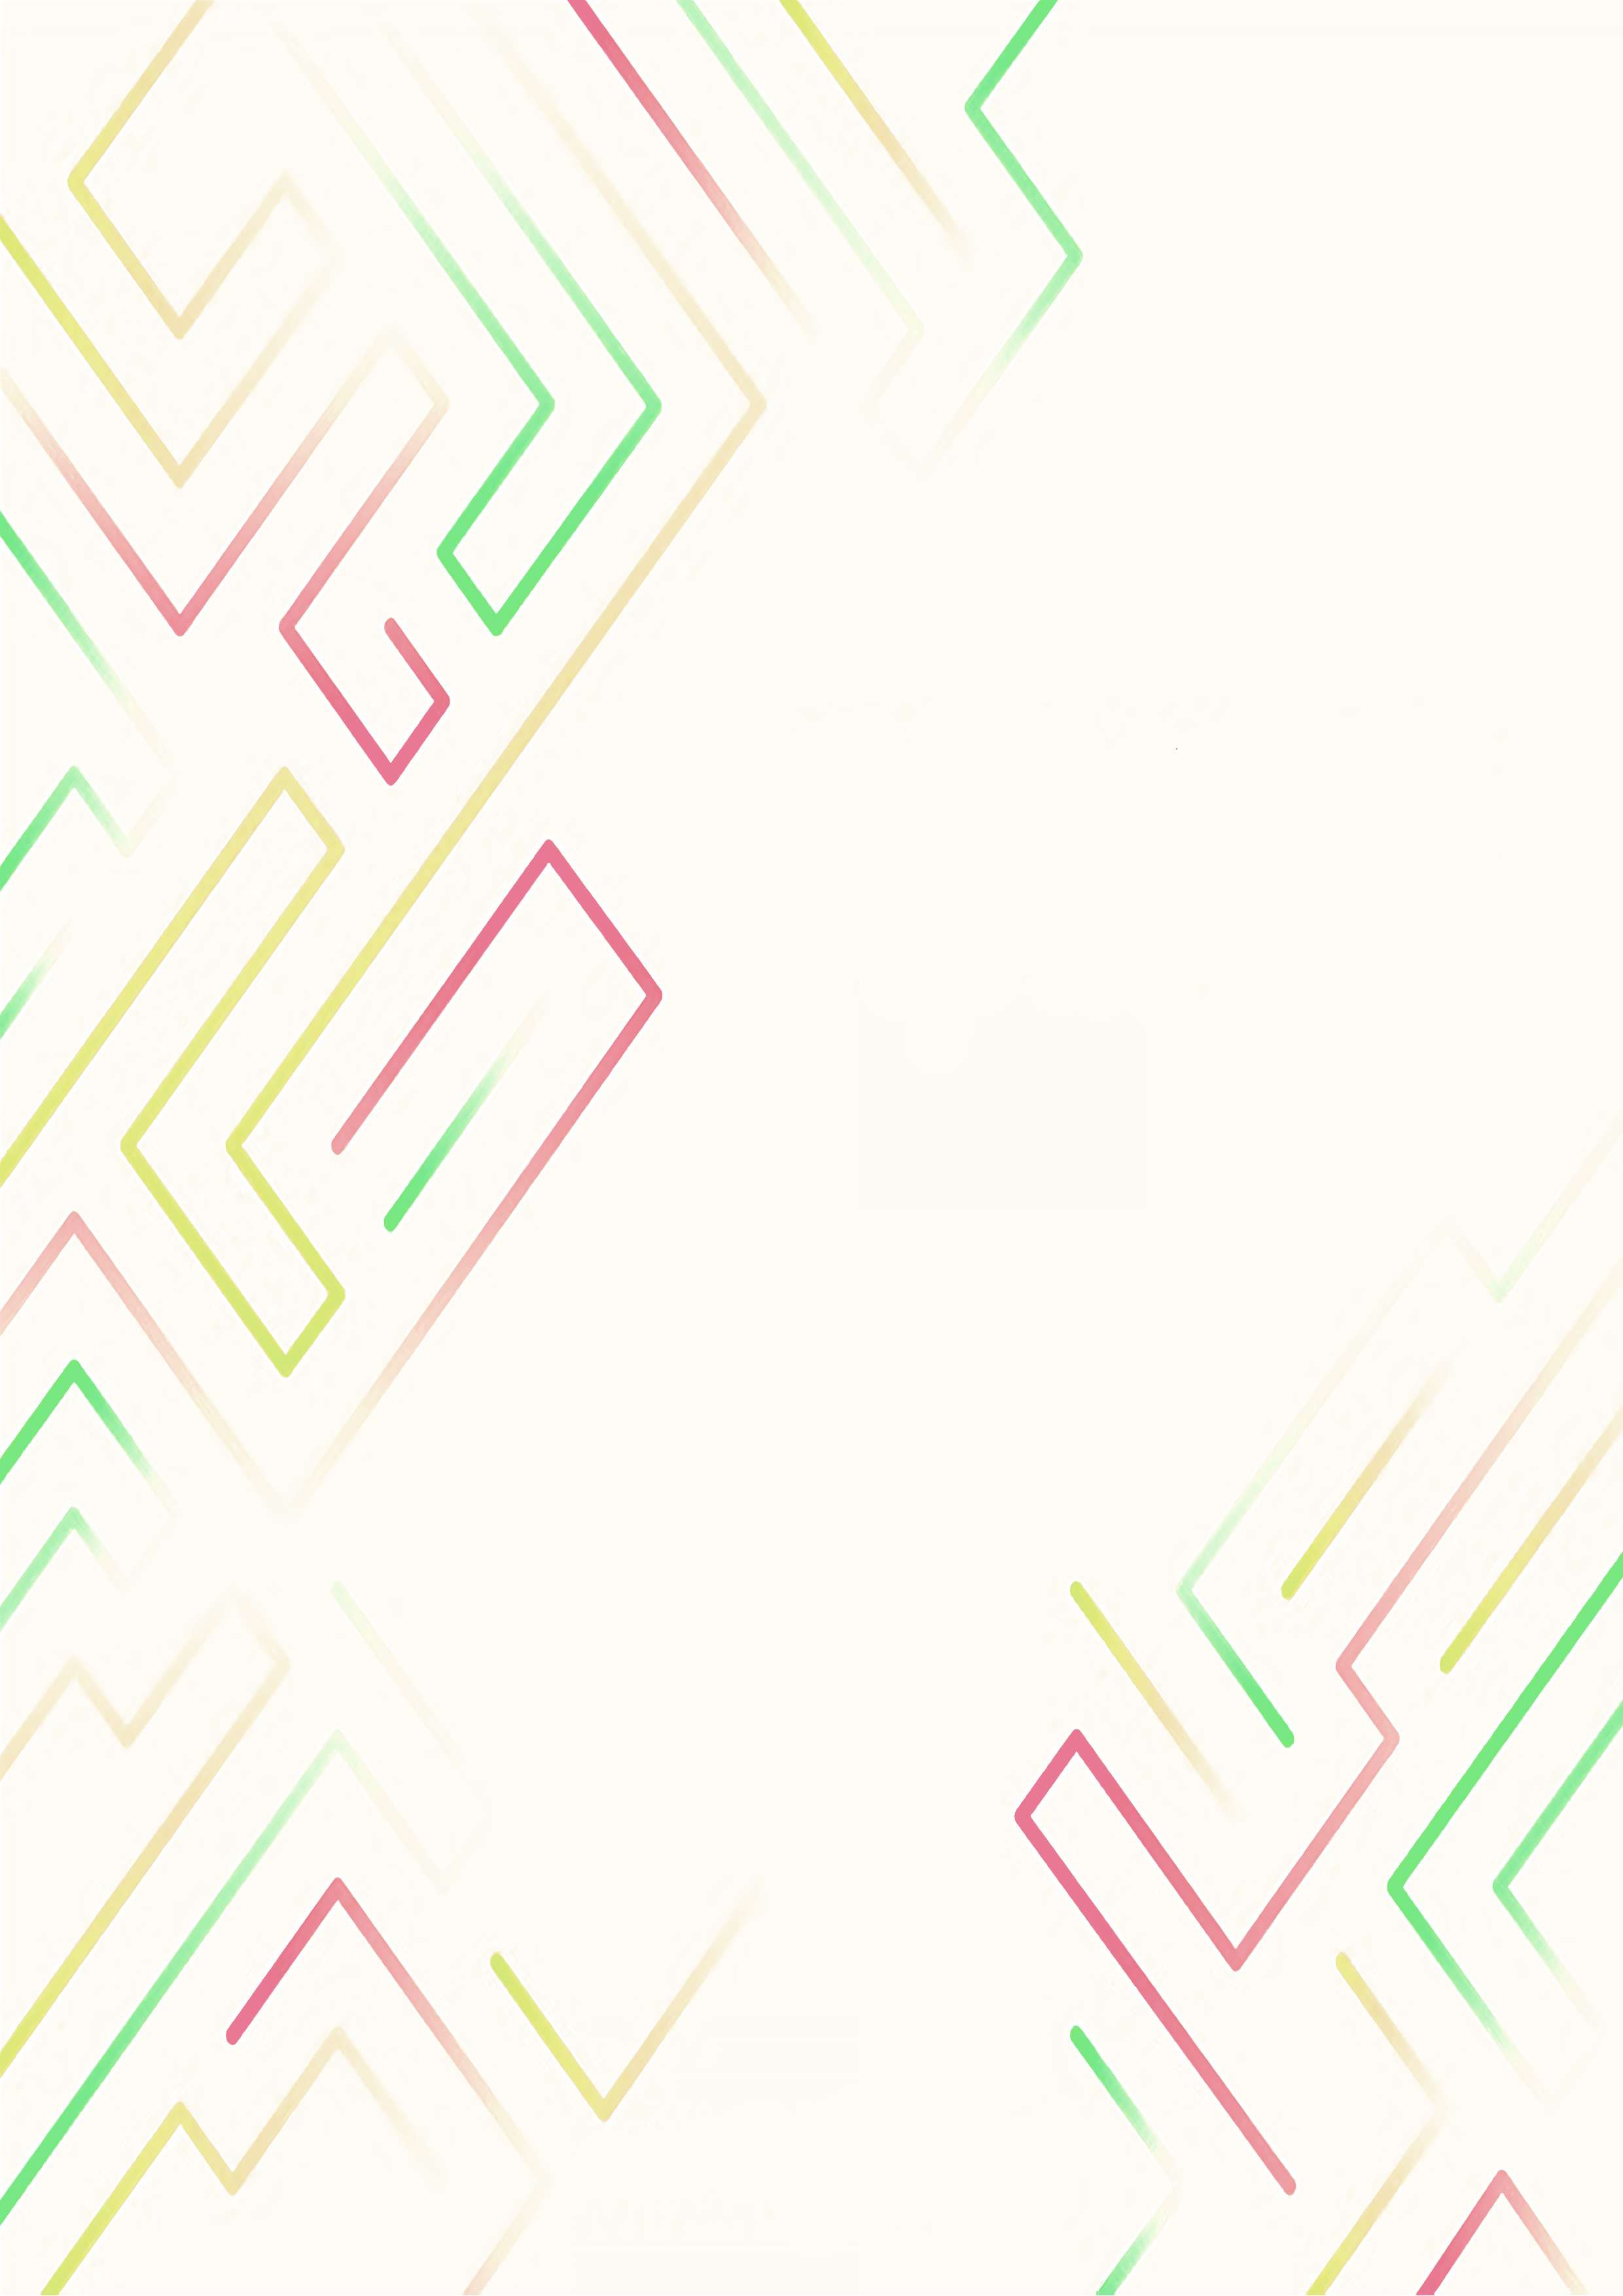
\includegraphics[width=\paperwidth,height=\paperheight]{wallpaper.png}
  }%
}

%configurando os hyperlinks
\hypersetup{
    colorlinks=true,
    linkcolor=blue,
    filecolor=magenta,      
    urlcolor=cyan,
}

%configurando os headers
\pagestyle{fancy}
\fancyhf{}
\rhead{LDO}
\lhead{Capítulo 1}
\rfoot{Página \thepage}

%configurando identação e separação de parágrafos
\parindent 1.27cm
\parskip   6pt

\flushbottom


%títulos,autor e datas
\title{\textbf{LDO - Capítulo 3\\
Como é feito esse aprendizado de máquina}}
\author{Homenique}
\date{23/10/2020}

%inicio do Texto 
\begin{document}
    \maketitle

    Quando vamos falar de Machine learning, é importante entendermos como as máquinas aprendem. de forma bem simples podemos dividir em 3 grupos de formas de aprendizados 
    \begin{itemize}
    \item 
    Aprendizado Supervisionado 
    \item Aprendizado Não supervisionado
    \item Aprendizado Por reforço
    \end{itemize}
    vamos conhecer um pouco de cada um?
    
%Texto 01
            \section*{\centering Aprendizado Supervisionado:}\label{sec:Aprendizado_Supervisionado}
            
            \begin{figure}[ht]
            \centering
            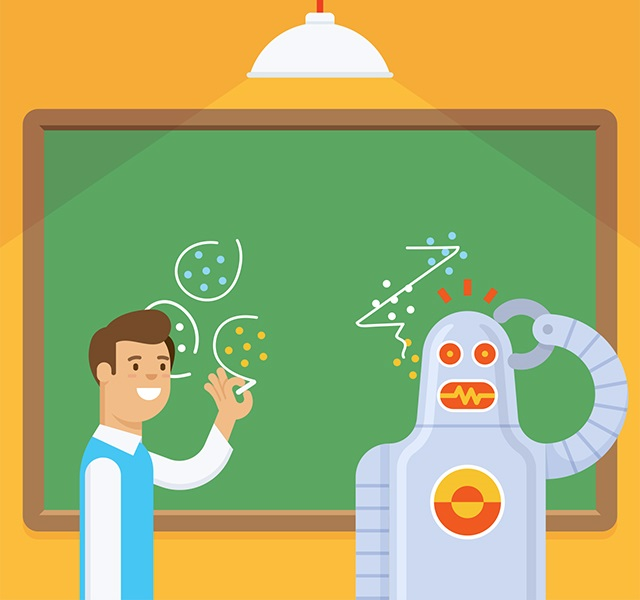
\includegraphics[scale=0.4]{robo_aprendedo.jpg}               
            \end{figure}
            

            \paragraph{}Aprendizagem supervisionada é a tarefa de encontrar uma função a partir de dados de treinamento rotulados. O objetivo é encontrar os parâmetros ótimos que ajustem um modelo que possa prever rótulos desconhecidos em outros objetos (o conjunto de teste). Se o rótulo é um número real, a tarefa chama-se regressão. Se o rótulo vem de um conjunto finito e não ordenado, então a tarefa chama-se classificação.
                
%Texto 02 
           \section*{\centering Não supervisionado:}
        
            \paragraph{}Na aprendizagem não-supervisionada temos menos informação sobre os objetos, em particular, o conjunto de treinamento não é rotulado. O nosso objetivo, neste contexto, é observar algumas similaridades entre os objetos e incluí-los em grupos apropriados. 
                
            \begin{figure}[ht]
            \label{fig:classificação}
            \centering
            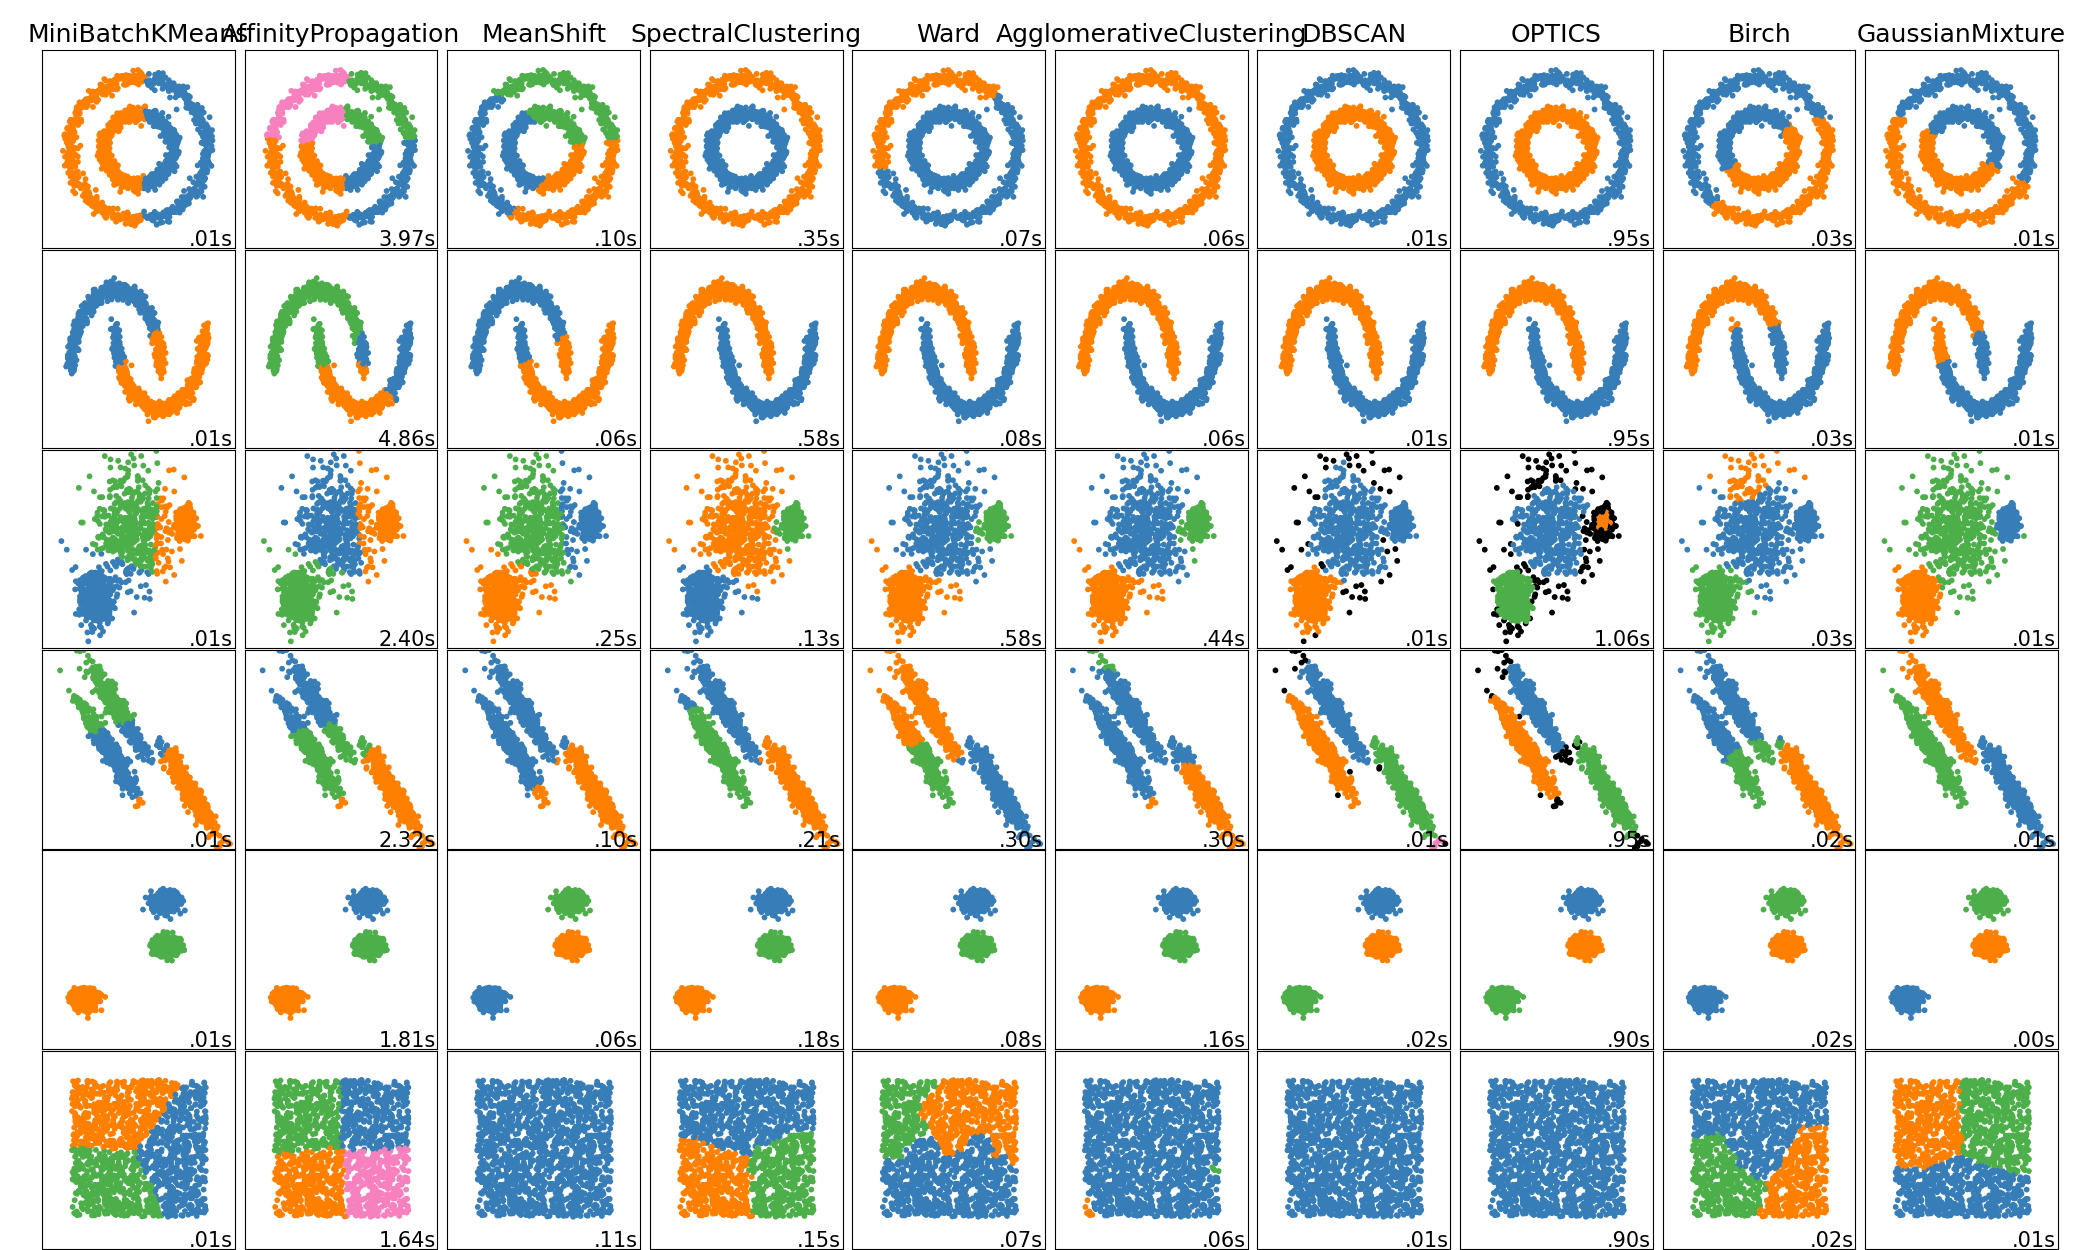
\includegraphics[scale=0.3]{classificação de grupos.png}               
            \end{figure}
            Alguns objetos podem diferir largamente de todos os grupos e, deste modo, podemos assumir que estes objetos são anomalias.
           
%Texto 03
           \clearpage
           \section*{\centering Por reforço:}
           \begin{figure}[ht]
           \centering
           
\includegraphics[scale=0.2]{jack-jack-num-num-cookie_orig.png}
           \end{figure}
   
           \paragraph{}Aprendizagem por reforço é uma área de aprendizagem de máquina que investiga como agentes de software devem agir em determinados ambientes de modo a maximizar alguma noção de recompensa cumulativa.


 %Iniciando listagem
        
            \section*{\centering Material extra}
            
            Que tal a gente ver algumas coisas a mais?
            \begin{itemize}
            
            %---------------------------------------
                \item\href{https://www.youtube.com/watch?v=R9OHn5ZF4Uo&t}{​How Machines Learn (com legendas em pt-br)}
            
            %----------------------------------------    
                \item\href{https://www.youtube.com/watch?v=mhe5e2B9bL8&t=1s}{Machine Learning: como ensinar uma máquina a aprender | Nerdologia Tech}
            
            %----------------------------------------
             \item Veja com ensinamento de máquina por reforço \\ %br 
             \href{https://www.youtube.com/watch?v=r8KWciNmEGw}{Inteligência Artificial ESTACIONANDO carros!}
            
            %----------------------------------------
             \item Uma explicação de como são pensados ensinamentos de máquina 
             \\ %br  
             \href{https://www.youtube.com/watch?v=aircAruvnKk}{But what is a Neural Network? | Deep learning, chapter 1}
            
            %----------------------------------------
             \item Um texto para você se aprofundar um pouco sobre esse tópico  
             \\ %br  
             \href{https://blog.wittel.com/o-que-e-machine-learning/}{O que é machine learning e quais são as suas aplicações no mercado?}
             
            \end{itemize}


        %Iniciando referências
        \begin{thebibliography}{2}
        %---------------------- Referencia 01 
        \bibitem{Nerdologia}
        Atila Iamarino
        \\
        \href{https://www.youtube.com/watch?v=mhe5e2B9bL8&t=1s}{Machine Learning: como ensinar uma máquina a aprender | Nerdologia Tech}
        
      %---------------------- Referencia 02
     
        \bibitem{CGP}
        CGP Grey \\
        \href{https://www.youtube.com/watch?v=R9OHn5ZF4Uo&t}{​How Machines Learn (com legendas em pt-br)}
     
     
        \end{thebibliography}
          

        
\end{document}